\chapter{Multivariate PMFs and Densities}
\label{mul}

Individual pmfs $p_X$ and densities $f_X$ don't describe correlations
betwen variables.  We need something more.  We need ways to describe
multivariate distributions.

\section{Multivariate Probability Mass Functions} 
\label{marblepmf}

Recall that for a single discrete random variable X, the distribution of
X was defined to be a list of all the values of X, together with the
probabilities of those values.  The same is done for a pair of discrete
random variables U and V, as follows.

Suppose we have a bag containing two yellow marbles, three blue ones and
four green ones.  We choose four marbles from the bag at random,
without replacement.  Let Y and B denote the number of yellow and blue
marbles that we get.  Then define the {\it two-dimensional} pmf of Y and
B to be

\begin{equation}
p_{Y,B}(i,j) = P(Y = i \textrm{ and } B = j) = 
\frac
{
\binom{2}{i}
\binom{3}{j}
\binom{4}{4-i-j}
}
{\binom{9}{4}}
\end{equation}

Here is a table displaying all the values of P(Y = i and B = j):

\begin{tabular}{|r|r|r|r|r|r|}
\hline
i $\downarrow$, j $\rightarrow$ & 0 & 1 & 2 & 3 \\ \hline 
0 & 0.0079 & 0.0952 & 0.1429 & 0.0317 \\ \hline 
1 & 0.0635 & 0.2857 & 0.1905 & 0.1587 \\ \hline 
2 & 0.0476 & 0.0952 & 0.0238 & 0.000 \\ \hline 
\end{tabular}

So this table is the distribution of the pair (Y,B).

Recall further that in the discrete case, we introduced a symbolic
notation for the distribution of a random variable X, defined as
$p_X(i) = P(X = i)$, where i ranged over all values that X takes on.
We do the same thing for a pair of random variables:

\begin{definition}
For discrete random variables U and V, their 
probability mass function is defined to be

\begin{equation}
p_{U,V}(i,j) = P(U = i \textrm{ and } V = j)
\end{equation}

where (i,j) ranges over all values taken on by (U,V).
Higher-dimensional pmfs are defined similarly, e.g.

\begin{equation}
p_{U,V,W}(i,j,k) = P(U = i \textrm{ and } V = j \textrm{ and } W = k)
\end{equation}
\end{definition}

So in our marble example above, $p_{Y,B}(1,2) = 0.048$, $p_{Y,B}(2,0) =
0.012$ and so on.

Just as in the case of a single discrete random variable X we have

\begin{equation}
P(X \in A) = \sum_{i \in A} p_X(i)
\end{equation}

for any subset A of the range of X, for a discrete pair (U,V) and any
subset A of the pair's range, we have

\begin{equation}
\label{probuva}
P[(U,V) \in A) =
\mathop{\sum \sum}_{(i,j) \in A} p_{U,V}(i,j)
\end{equation}

Again, consider our marble example.  Suppose we want to find $P(Y < B)$.
Doing this ``by hand,'' we would simply sum the relevant probabilities 
in the table above, which are marked in bold face below:

\begin{tabular}{|r|r|r|r|r|r|}
\hline
i $\downarrow$, j $\rightarrow$ & 0 & 1 & 2 & 3 \\ \hline 
0 & 0.002 & {\bf 0.024} & {\bf 0.036} & {\bf 0.008} \\ \hline 
1 & 0.162 & 0.073 & {\bf 0.048} & {\bf 0.004} \\ \hline 
2 & 0.012 & 0.024 & 0.006 & {\bf 0.000} \\ \hline 
\end{tabular}

The desired probability would then be 0.024+0.036+0.008+0.048+0.004 =
0.12.

Writing it in the more formal way using (\ref{probuva}), we would set

\begin{equation}
A = \{ (i,j): i < j \}
\end{equation}

and then

\begin{equation}
\label{probyltb}
P(Y < B) = 
P[(Y,B) \in A) =
\sum_{i=0}^2 
\sum_{j=i+1}^3
p_{Y,B}(i,j)
\end{equation}

Note that the lower bound in the inner sum is j = i+1.  This reflects
the common-sense point that in the event $Y < B$, B must be at least
equal to Y+1.

Of course, this sum still works out to 0.12 as before, but it's
important to be able to express this as a double sum of $p_{Y,B}()$, as
above.  We will rely on this to motivate the continuous case in the next
section.

Expected values are calculated in the analogous manner.  Recall that for
a function g() of X

\begin{equation}
E[g(X] = \sum_{i} g(i) p_{X}(i)
\end{equation}

So, for any function g() of two discrete random variables U and V,
define

\begin{equation}
E[g(U,V)] = 
\sum_i \sum_j g(i,j) p_{U,V}(i,j)
\end{equation}

For instance, if for some bizarre reason we wish to find the expected
value of the product of the numbers of yellow and blue marbles
above,\footnote{Not so bizarre, we'll find in Section \ref{covar}.}, the
calculation would be

\begin{equation}
E(YB) = \sum_{i=0}^2 \sum_{j=0}^{3} i j ~ p_{Y,B}(i,j)
= 0.255
\end{equation}

The univariate pmfs, called {\it marginal pmfs}, can of course be
recovered from the multivariate pmf:

\begin{equation}
\label{uvmarg}
p_U(i) = P(U = i) = \sum_{j} P(U = i, V = j) =
\sum_{j} p_{U,V}(i,j)
\end{equation}

For example, look at the table following (\ref{probuva}).  Evaluating
(\ref{uvmarg}) for i = 1, say, with U = Y and V = B, would give us
0.012 + 0.024 + 0.006 + 0.000 = 0.042.  Then all that (\ref{uvmarg})
tells us is the P(Y = 1) = 0.042, which is obvious from the table;
(\ref{uvmarg}) simply is an application of our old principle, ``Break
big events down into small events.''

Needless to say, we can recover the marginal distribution of V similarly
to (\ref{uvmarg}):

\begin{equation}
p_V(j) = P(V = j) = \sum_{i} P(U = i, V = j) =
\sum_{i} p_{U,V}(i,j)
\end{equation}

\section{Multivariate Densities}

\subsection{Motivation and Definition}

Extending our previous definition of cdf for a single variable, we
define the two-dimensional cdf for a pair of random variables X and Y
(discrete or continuous) as

\begin{equation}
F_{X,Y}(u,v) = P(X \leq u {\rm ~and~ } Y \leq v)
\end{equation}

If X and Y were discrete, we would evaluate that cdf via a double sum of
their bivariate pmf.  You may have guessed by now that the analog for
continuous random variables would be a double integral, and it is.  The
integrand is the bivariate density:

\begin{equation}
f_{X,Y} (u,v) = \frac{\partial^2}{\partial u \partial v}
F_{X,Y}(u,v)
\end{equation}

Densities in higher dimensions are defined similarly.\footnote{Just as
we noted in Section \ref{mixed} that some random variables are neither
discrete nor continuous, there are some pairs of continuous random
variables whose cdfs do not have the requisite derivatives.  We will not
pursue such cases here.}

As in the univariate case, a bivariate density shows which regions of
the X-Y plane occur more frequently, and which occur less frequently.

\subsection{Use of Multivariate Densities in Finding Probabilities
and Expected Values}

Again by analogy, for any region A in the X-Y plane,

\begin{equation}
\label{probina}
P[(X,Y) \epsilon A] 
= \iint \limits_A f_{X,Y} (u,v) ~ du ~ dv
\end{equation}

So, just as probabilities involving a single variable X are found by
integrating $f_X$ over the region in question, for probabilities
involving X and Y, we take the double integral of $f_{X,Y}$ over that
region.

Also, for any function g(X,Y), 

\begin{equation}
\label{meancontin}
E[g(X,Y)] 
= \int_{-\infty}^{\infty} \int_{-\infty}^{\infty} g(u,v) f_{X,Y} (u,v) ~ du ~ dv
\end{equation}

where it must be kept in mind that $f_{X,Y}(u,v)$ may be 0 in some
regions of the U-V plane.  Note that there is no set A here as in
(\ref{probina}).  See (\ref{eofsqrt}) below for an example.

Finding marginal densities is also analogous to the discrete case, e.g.

\begin{equation}
\label{contmarg}
f_X(s) = \int_{t} f_{X,Y} (s,t)  ~ dt
\end{equation}

Other properties and calculations are analogous as well.  For instance,
the double integral of the density is equal to 1, and so on.

\subsection{Example: a Triangular Distribution}
\label{8st}

Suppose (X,Y) has the density 

\begin{equation}
\label{tridens}
f_{X,Y}(s,t) = 8st, ~ 0 < t < s < 1
\end{equation}

The density is 0 outside the region $0 < t < s < 1$.

First, think about what this means, say in our notebook context.  We do
the experiment many times.  Each line of the notebook records the values
of X and Y.  Each of these (X,Y) pairs is a point in the triangular region
$0 < t < s < 1$.  Since the density is highest near the point (1,1) and
lowest near (0,0), (X,Y) will be observed near (1,1) much more often
than near (0,0), with points near, say, (1,0.5) occurring with middling
frequencies.  

Let's find $P(X+Y > 1)$.  This calculation will involve a double
integral.  The region A in (\ref{probina}) is $\{(s,t): s+t > 1, 0 < t <
s < 1\}$.  We have a choice of integrating in the order ds dt or dt ds.
The latter will turn out to be more convenient.

To see how the limits in the double integral are obtained, first review
(\ref{probyltb}).  We use the same reasoning here, changing from sums to
integrals and applying the current density, as shown in this figure:

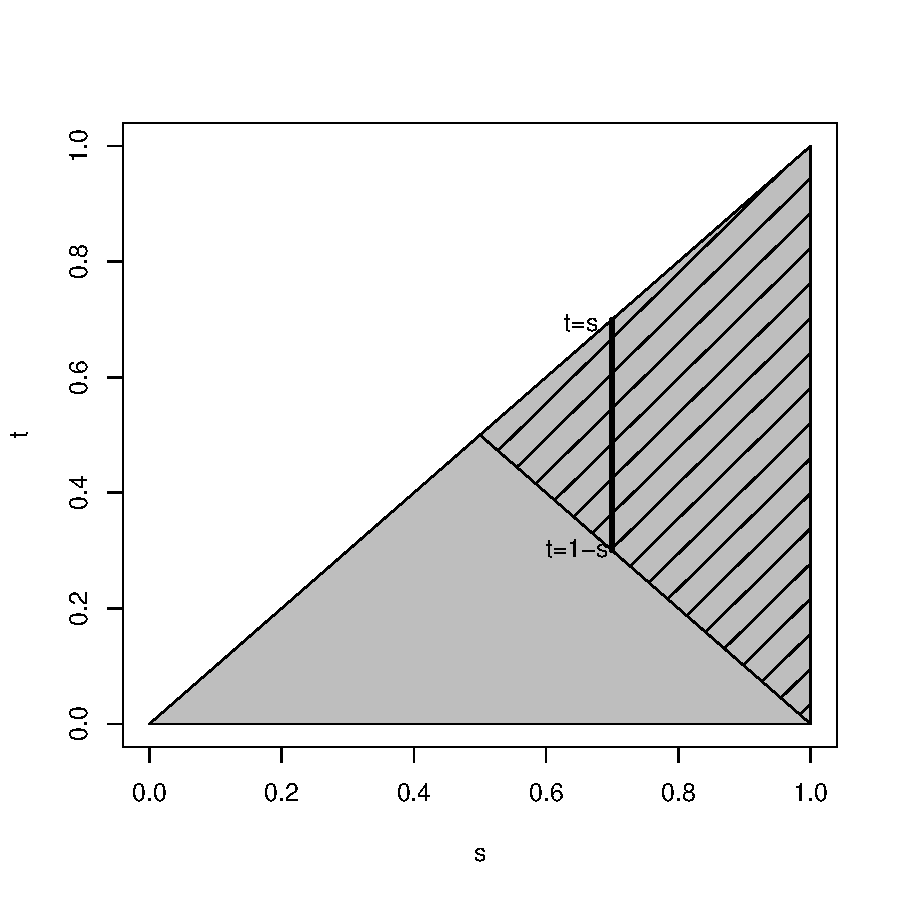
\includegraphics[width=4in]{DoubleInt.pdf}

% Note to me:  The code for generating this figure is at the end of this
% .tex document.

Here s represents X and t represents Y.  The gray area is the region in
which (X,Y) ranges.  The subregion A in (\ref{probina}), corresponding
to the event X+Y $>$ 1, is shown in the striped area in the figure.

The dark vertical line shows all the points (s,t) in the striped region
for a typical value of s in the integration process.  Since s is the
variable in the outer integral, considered it fixed for the time being
and ask where t will range {\it for that s}.  We see that for X = s, Y
will range from 1-s to s; thus we set the inner integral's limits to 1-s
and s.  Finally, we then ask where s can range, and see from the picture
that it ranges from 0.5 to 1.  Thus those are the limits for the outer
integral.

\begin{equation}
\label{xygt1}
P(X+Y > 1) = \int_{0.5}^{1} \int_{1-s}^{s} 8st ~ dt ~ ds
= \int_{0.5}^{1} 8s \cdot (s-0.5) ~ ds = \frac{5}{6}
\end{equation}

Following (\ref{meancontin}), 

\begin{equation}
\label{eofsqrt}
E[\sqrt{X+Y}] = \int_{0}^{1} \int_{0}^{s} \sqrt{s+t} ~ 8st ~ dt ~ ds
\end{equation}

Let's find the marginal density $f_Y(t)$.  Just as we ``summed out'' in
(\ref{uvmarg}), in the continuous case we must ``integrate out'' the s
in (\ref{tridens}):

\begin{equation}
\label{ydens}
f_Y(t) = \int_{t}^{1} 8st ~ ds = 4t - 4t^3
\end{equation}

for $0 < t < 1$, 0 elsewhere.

Let's find the correlation between X and Y for this density. 

\begin{eqnarray}
E(XY) &=& 
\int_{0}^{1} \int_{0}^{s} st \cdot 8st ~ dt ~ ds \\
&=& \int_{0}^{1} 8s^2 \cdot s^3/3 ~ ds \\
&=& \frac{4}{9}
\end{eqnarray}

\begin{eqnarray}
f_X(s) &=& \int_{0}^{s} 8st ~ dt \\ 
&=& 4s t^2 \Big |_0^s \\
&=& 4s^3 
\end{eqnarray}

\begin{eqnarray}
f_Y(t) &=& \int_{t}^{1} 8st ~ ds \\ 
&=& 4t \cdot s^2 \Big |_t^1 \\
&=& 4t (1-t^2)
\end{eqnarray}

\begin{equation}
EX = \int_{0}^{1} s \cdot 4s^3 ~ ds  = \frac{4}{5}
\end{equation}

\begin{equation}
E(X^2) = \int_{0}^{1} s^2 \cdot 4s^3 ~ ds  = \frac{2}{3}
\end{equation}

\begin{equation}
Var(X) =  \frac{2}{3} - \left (\frac{4}{5} \right )^2 = 0.027
\end{equation}

\begin{equation}
EY = \int_{0}^{1} t \cdot (4t-4t^3)  ~ ds  
= \frac{4}{3} - \frac{4}{5}
= \frac{8}{15}
\end{equation}

\begin{equation}
E(Y^2) = \int_{0}^{1} t^2 \cdot (4t-4t^3) ~ dt  = 
1 - \frac{4}{6} = \frac{1}{3}
\end{equation}

\begin{equation}
Var(Y) =  \frac{1}{3} - \left (\frac{8}{15} \right )^2 = 0.049
\end{equation}

\begin{equation}
Cov(X,Y) = \frac{4}{9} - \frac{4}{5} \cdot \frac{8}{15} = 0.018
\end{equation}

\begin{equation}
\rho(X,Y) = \frac{0.018}{\sqrt{0.027 \cdot 0.049}} = 0.49
\end{equation}

\subsection{Example:  Train Rendezvouz}

Train lines A and B intersect at a certain transfer point, with the
schedule stating that trains from both lines will arrive there at 3:00
p.m.  However, they are often late, by amounts $X$ and $Y$, measured in
hours, for the two trains.  The bivariate density is

\begin{equation}
f_{X,Y}(s,t) = 2 - s -t, ~ 0 < s,t < 1
\end{equation}

Two friends agree to meet at the transfer point, one taking line A and
the other B.  Let $W$ denote the time in minutes the person arriving on
line B must wait for the friend.  Let's find $P(W > 6)$.

First, convert this to a problem involving X and Y, since they are the
random variables for which we have a density, and then use (\ref{probina}):

\begin{eqnarray}
P(W > 0.1) &=& P(Y + 0.1 < X ) \\
&=& \int_{0.1}^{1}   
\int_{0}^{s-0.1} (2-s-t) ~ dt ds
\end{eqnarray}

\section{More on Sets of Independent Random Variables}

\subsection{Probability Mass Functions and Densities Factor in the
Independent Case}
\label{theyfactor}

If X and Y are independent, then 

\begin{equation}
\label{indeppmf}
p_{X,Y} = p_X p_Y
\end{equation}

in the discrete case, and 

\begin{equation}
\label{indepdens}
f_{X,Y} = f_X f_Y
\end{equation}

in the continuous case.  In other words, the joint pmf/density is the
product of the marginal ones.

This is easily seen in the discrete case:

\begin{eqnarray}
p_{X,Y}(i,j) 
&=& P(X = i \textrm{ and } Y = j) ~~ (\textrm{definition}) \\
&=& P(X = i) P(Y = j)  ~~ (\textrm{independence}) \\
&=& p_X(i) p_Y(j)  ~~ (\textrm{definition)})
\end{eqnarray}

Here is the proof for the continuous case; 

\begin{eqnarray}
f_{X,Y} (u,v) 
&=& \frac{\partial^2}{\partial u \partial v}
 F_{X,Y}(u,v) \\
&=& \frac{\partial^2}{\partial u \partial v}
 P(X \leq u
\textrm{ and } Y \leq v) \\
&=& \frac{\partial^2}{\partial u \partial v}
\left [ P(X \leq u)
\cdot P(Y \leq v) \right ] \\
&=& \frac{\partial^2}{\partial u \partial v}
 F_X(u) 
\cdot F_Y(v) \\
&=& f_X(u) f_Y(v)
\end{eqnarray}

\subsection{Convolution} 
\label{convolution}

\begin{definition}
Suppose g and h are densities of continuous random
variables X and Y, respectively.  The {\bf convolution} of g and h,
denoted g*h,\footnote{The reason for the asterisk, suggesting a product,
will become clear in Section \ref{tranfssums}.} is another density,
defined to be that of the random variable X+Y.  In other words,
convolution is a binary operation on the set of all densities.

If X and Y are nonnegative and independent, then the convolution reduces to 

\begin{equation}
\label{convcontin}
f_Z(t) = \int_{0}^t g(s) h(t-s) ~ ds
\end{equation}
\end{definition}

You can get intuition on this by considering the discrete case.  Say U
and V are nonnegative integer-valued random variables, and set W = U+V.
Let's find $p_W$;

\begin{eqnarray}
\label{convdiscleft}
p_W(k) &=& P(W = k) ~~ (\textrm{by definition}) \\ 
&=& P(U + V = k) ~~ (\textrm{substitution}) \\
&=& \sum_{i=0}^k P(U = i \textrm{ and } V = k-i) ~~ (\textrm{``In what ways can it happen?''}) \\
&=& \sum_{i=0}^k p_{U,V}(i,k-i) ~~ (\textrm{by definition}) \\
&=& \sum_{i=0}^k p_U(i) p_V(k-i)  ~~ (\textrm{from Section \ref{theyfactor}})
\label{convdiscright}
\end{eqnarray}

Review the analogy between densities and pmfs in our unit on continuous
random variables, Section \ref{densitymotivation}, and then see how
(\ref{convcontin}) is analogous to (\ref{convdiscleft}) through
(\ref{convdiscright}):  

\begin{itemize}

\item k in  
(\ref{convdiscleft})
is analogous to t in 
(\ref{convcontin}) 

\item the limits 0 to k in  
(\ref{convdiscright})
are analogous to the limits 0 to t in 
(\ref{convcontin}) 

\item the expression k-i in  
(\ref{convdiscright})
is analogous to t-s in 
(\ref{convcontin}) 

\item and so on

\end{itemize}

\subsection{Example:  Ethernet}
\label{ethernetex}

Consider this network, essentially Ethernet.  Here nodes can send at any
time.  Transmission time is 0.1 seconds.  Nodes can also ``hear'' each
other; one node will not start transmitting if it hears that another has
a transmission in progress, and even when that transmission ends, the
node that had been waiting will wait an additional random time, to
reduce the possibility of colliding with some other node that had been
waiting.

Suppose two nodes hear a third transmitting, and thus refrain from
sending.  Let X and Y be their random backoff times, i.e. the random
times they wait before trying to send.  (In this model, assume that they
do not do ``listen before talk'' after a backoff.) Let's find the
probability that they clash, which is $P(|X - Y| \leq 0.1)$.  

Assume that X and Y are independent and exponentially distributed with
mean 0.2, i.e. they each have density $5e^{-5u}$ on $(0,\infty)$.
Then from (\ref{indepdens}), we know that their joint density
is the product of their marginal densities, 

\begin{equation}
f_{X,Y}(s,t) = 25 e^{-5(s+t)}, s,t > 0
\end{equation}

Now

\begin{equation}
P(|X - Y| \leq 0.1) = 1 - P(|X - Y| > 0.1)
= 1 - P(X > Y + 0.1) - P(Y > X + 0.1) 
\end{equation}

Look at that first probability.  Applying (\ref{probina}) with $A =
\{(s,t): s > t + 0.1, 0 < s,t\}$, we have

\begin{equation}
P(X > Y + 0.1) =
\int_{0}^{\infty} \int_{t+0.1}^{\infty} 25 e^{-5(s+t)} ~ ds ~ dt = 0.303
\end{equation}

By symmetry, $P(Y > X + 0.1)$ is the same.  So, the probability of a
clash is 0.394, rather high.  We may wish to increase our mean backoff
time, though a more detailed analysis is needed.

\subsection{Example:  Analysis of Seek Time}

This will be an analysis of seek time on a disk.  Suppose we have mapped
the innermost track to 0 and the outermost one to 1, and assume that (a)
the number of tracks is large enough to treat the position H of the
read/write head the interval [0,1] to be a continous random variable,
and (b) the track number requested has a uniform distribution on that
interval.

Consider two consecutive service requests for the disk, denoting their
track numbers by X and Y.  In the simplest model, we assume that X and Y
are independent, so that  the joint distribution of X and Y is the
product of their marginals, and is thus is equal to 1 on the square $0
\leq X,Y \leq 1$.

The seek distance will be $|X-Y|$.  Its mean value is found by taking
g(s,t) in (\ref{meancontin}) to be $|s-t|$.

\begin{equation}
\int_{0}^{1} \int_{0}^{1} |s-t| \cdot 1 ~ ds ~ dt = \frac{1}{3}
\end{equation}

Let's find the density of the seek time $S = |X-Y|$:

\begin{eqnarray}
F_S(v) &=& P(|X-Y| \leq v) \\
&=& P(-v \leq X-Y \leq v) \\ 
&=& 1 - P(X-Y < -v) - P(X-Y > v) \\
&=& 1 - (1-v)^2
\end{eqnarray}

where for instance $P(X - Y > v)$ the integral of 1 on the triangle with
vertices (v,0), (1,0) and (1,1-v), thus equal to the area of that
triangle, $0.5 (1-v)^2$.

Then

\begin{equation}
f_S(v) = \frac{d}{dt} F_S(v) = 2(1-v)
\end{equation}

By the way, what about the assumptions here?  The independence would be
a good assumption, for instance, for a heavily-used file server accessed
by many different machines.  Two successive requests are likely to be
from different machines, thus independent.  In fact, even within the
same machine, if we have a lot of users at this time, successive
requests can be assumed independent.  On the other hand, successive
requests from a particular user probably can't be modeled this way.

As mentioned in our unit on continuous random variables, page
\pageref{defrag}, if it's been a while since we've done a defragmenting
operation, the assumption of a uniform distribution for requests is
probably good.

Once again, this is just scratching the surface.  Much more
sophisticated models are used for more detailed work.

\subsection{Example:  Backup Battery}
\label{backup}

Suppose we have a portable machine that has compartments for two
batteries. The main battery has lifetime X with mean 2.0 hours, and the
backup's lifetime Y has mean life 1 hours. One replaces the first by
the second as soon as the first fails. The lifetimes of the batteries
are exponentially distributed and independent. Let's find the density of
W, the time that the system is operational (i.e. the sum of the
lifetimes of the two batteries).

Recall that if the two batteries had the same mean lifetimes, W would
have a gamma distribution.  But that's not the case here.  But we notice
that the distribution of W is a convolution of two exponential
densities, as it is the sum of two nonnegative independent random
variables.  Using (\ref{convolution}), we have

\begin{equation}
f_W(t) = \int_{0}^t f_X(s) f_Y(t-s) ~ ds
= \int_{0}^t 0.5e^{-0.5s} e^{-(t-s)}~ ds
= e^{-0.5t} - e^{-t}, ~ 0 < t < \infty
\end{equation}

\subsection{Example:  Minima of Uniformly Distributed Random Variables}
\label{minunif}

Suppose X and Y be independent and each have a uniform distribution on
the interval (0,1).  Let Z = min(X,Y).  Find $f_Z$:

\begin{eqnarray}
F_{Z}(t) &=& P(Z \leq t) ~~~~ \textrm{(def. of cdf) }\\
&=& 1-P(Z>t) \\
&=& 1-P(X > t \textrm{ and } Y > t)  ~~~~
\textrm{(min(u,v) $> t$ iff both u,v $> t$)} \\
&=& 1 - P(X > t) P(Y > t) ~~~~ \textrm{(indep.) }\\
&=& 1 - (1-t)^2 ~~~~ \textrm{(indep.) }\\
\end{eqnarray}

The density of Z is then the derivative of that last expression:

\begin{equation}
f_Z(t) = 2(1-t), ~~~~ 0 < t < 1 
\end{equation}

\subsection{Example:  Ethernet Again}

In the Ethernet example in Section \ref{ethernetex}, we assumed that
transmission time was a constant, 0.1.  Now let's account for messages
of varying sizes, by assuming that transmission time T for a message is
random, exponentially distributed with mean 0.1.  Let's find $P(X < Y
\textrm{ and there is no collision})$.

That probability is equal to $P(X+T < Y)$.   Well, this sounds like
we're going to have to deal with triple integrals, but actually not.
The derivation in Section \ref{backup} shows that the density of S = X+T 
is

\begin{equation}
f_{S}(t) = e^{-0.1t} - e^{-0.2t}, ~ 0 < t < \infty
\end{equation}

Thus the joint density of S and Y is 

\begin{equation}
f_{S,Y}(u,v) = (e^{-0.1u} - e^{-0.2u}) 0.2e^{-0.2v}, ~~ 0 < u,v, <
\infty
\end{equation}

We can then evaluate $P(S < Y)$ as a double integral, along the same
lines as we did for instance in (\ref{xygt1}).

\section{Example:  Finding the Distribution of the Sum of Nonindependent
Random Variables}

In Section \ref{convolution}, we found a general formula for the
distribution of the sum of two independent random variables.  What about
the nonindependent case?

Suppose for instance $f_{X,Y}(s,t) = 2$ on $0 < t < s < 1$, 0 elsewhere.
Let's find $f_{X+Y}(w)$ for the case $0 < w < 1$.

Since X and Y are not independent, we cannot use convolution.  But:

\begin{eqnarray}
F_{X+Y}(w) &=& P(X+Y) \leq w\\
&=&
\int_{0}^{w/2}
\int_{t}^{w-t} 2 ~ ds ~ dt \\
&=& w^2 / 2
\end{eqnarray}

So $f_{X+Y}(w) = w$.

The case $1 < w < 2$ is similar.

\section{Parametric Families of Multivariate Distributions}

Since there are so many ways in which random variables can correlate
with each other, there are rather few parametric families commonly used
to model multivariate distributions (other than those arising from sets
of independent random variables have a distribution in a common
parametric univariate family).  We will discuss two here.

\subsection{The Multinomial Family of Distributions}

\subsubsection{Probability Mass Function}
\label{multinompmfsection}

This is a generalization of the binomial family.

Suppose one rolls a die 8 times.  What is the probability that the
results consist of two 1s, one 2, one 4, three 5s and one 6?  Well, if
the rolls occur in that order, i.e. the two 1s come first, then the 2,
etc., then the probability is 

\begin{equation}
\left (\frac{1}{6} \right )^2
\left (\frac{1}{6} \right )^1
\left (\frac{1}{6} \right )^0
\left (\frac{1}{6} \right )^1
\left (\frac{1}{6} \right )^3
\left (\frac{1}{6} \right )^1
\end{equation}

But there are many different orderings, in fact

\begin{equation}
\frac{8!}{2!1!0!1!3!1!}
\end{equation}

of them, from Section \ref{multnomcoeff}, and thus 

\begin{equation}
P(\textrm{two 1s, one 2, no 3s, one 4, three 5s, one 6}) =
\frac{8!}{2!1!0!1!3!1!}
\left (\frac{1}{6} \right )^2
\left (\frac{1}{6} \right )^1
\left (\frac{1}{6} \right )^0
\left (\frac{1}{6} \right )^1
\left (\frac{1}{6} \right )^3
\left (\frac{1}{6} \right )^1
\end{equation}

From this, we can more generally see the following.  Suppose:

\begin{itemize}

\item we have n trials, each of which has r possible
outcomes or categories

\item the trials are independent

\item the i$^{th}$ outcome has probability $p_i$

\end{itemize}

Let $X_i$ denote the number of trials with outcome i, i = 1,...,r.  In
the die example above, for instance, r = 6 for the six possible outcomes
of one trial, i.e. one roll of the die, and $X_1$ is the number of times
we got one dot, in our n = 8 rolls.

Then we say that the vector $X = (X_1,...,X_r)$ have a {\bf multinomial
distribution}.  Since the $X_i$ are discrete random variables, they have
a joint pmf $p_{X_1,...,X_r}()$.  Taking the above die example for
illustration again, the probability of interest there is
$p_{X}(2,1,0,1,3,1)$.  We then have in general,

\begin{equation}
\label{multinompmf}
p_{X_1,...,X_r}(j_1,...,j_r) =
\frac
{n!}
{j_1!...j_r!}
p_1^{j_1}...  p_r^{j_r}
\end{equation}

Note that this family of distributions has r+1 parameters:  n and the
$p_i$.  Of course, you might count it as only r, since the $p_i$ sum to
one and thus are not free of each other.

R has the function {\bf dmultinom()} for the multinomial pmf.  The call
{\bf dmultinom(x,n,prob)} evaluates (\ref{multinompmf}), where
{\bf x} is the vector $(j_1,...,j_r)$ and {\bf prob} is $(p_1,...,p_r)$
.

We can simulate multinomial random vectors in R using the {\bf sample()} 
function:

\begin{Verbatim}[fontsize=\relsize{-2},numbers=left]
# n is the number of trials, p the vector of probabilities of the r
# categories
multinom <- function(n,p) {
   r <- length(p)
   outcome <- sample(x=1:r,size=n,replace=T,prob=p)
   counts <- vector(length=r)  # counts of the various categories
   # tabulate the counts (could be done more efficiently)
   for (i in 1:n) {
       j <- outcome[i] 
       counts[j] <- counts[j] + 1
   }
   return(counts)
}
\end{Verbatim}

\subsubsection{Example:  Component Lifetimes}

Say the lifetimes of some electronic component, say a disk drive, are
exponentially distributed with mean 4.5 years.  If we have six of them, what
is the probability that two fail before 1 year, two last between 1 and 2
years, and the remaining two last more than 2 years?

Let (X,Y,Z) be the number that last in the three time intervals.  Then
this vector has a multinomial distribution, with n = 6 trials, and

\begin{equation}
p_1 = \int_{0}^{1} \frac{1}{4.5} e^{-t/4.5} ~ dt = 0.20
\end{equation}

\begin{equation}
p_2 = \int_{1}^{2} \frac{1}{4.5} e^{-t/4.5} ~ dt = 0.16
\end{equation}

\begin{equation}
p_3 = \int_{2}^{\infty} \frac{1}{4.5} e^{-t/4.5} ~ dt = 0.64
\end{equation}

We then use (\ref{multinompmf}) to find the specified probability, which
is:

\begin{equation}
\frac{6!}{2!2!2!} ~
0.20^2
0.16^2
0.64^2
\end{equation}

\subsubsection{Mean Vectors and Covariance Matrices in the Multinomial
Family}

Consider a multinomially distributed random vector $X = (X_1,...,X_r)'$,
with n trials and category probabilities $p_i$.  Let's find its mean
vector and covariance matrix.

First, note that the marginal distributions of the $X_i$ are binomial!
So, 

\begin{equation}
\label{multinommeanvar}
EX_i = np_i \textrm{ and } Var(X_i) = np_i(1-p_i)
\end{equation}

So we know EX now:

\begin{equation}
EX = 
\left (
\begin{array}{c}
np_1 \\
... \\
np_r
\end{array}
\right )
\end{equation}

We also know the diagonal elements of Cov(X)---$np_i(1-p_i)$ is the
i$^{th}$ diagonal element, i = 1,...,r.  

But what about the rest?  The derivation will follow in the footsteps of
those of (\ref{binvar}), but now in a vector context.  Prepare to use
your indicator random variable, random vector and covariance matrix
skills!  Also, this derivation will really build up your ``probabilistic
stamina level.''  So, it's good for you!  But {\bf now is the time to review
(\ref{binvar}), Section \ref{indicator} and Section \ref{matrix}, before
continuing.}  

We'll continue the notation of the last section.  In order to keep on
eye on the concrete, we'll often illustrate the notation with the die
example above; there we rolled a die 8 times, and defined 6 categories
(one dot, two dots, etc.).  We were interested in probabilities
involving the number of trials that result in each of the 6 categories.

Define the random vector $T_i$ to be the outcome of the i$^{th}$ trial.
It is a vector of indicator random variables, one for each of the r
categories.  In the die example, for instance, consider the second roll,
which is recorded in $T_2$.  If that roll turns out to be, say, 5, then

\begin{equation}
T_2 =
\left ( \begin{array}{r} 
0 \\
0 \\
0 \\
0 \\
1 \\
0 \\
\end{array} \right )
\end{equation}

Here is the key observation:

\begin{equation}
\label{multinomsumindic}
\left ( \begin{array}{r}
X_1 \\
... \\
X_r \\
\end{array} \right )
=
\sum_{i=1}^n T_i
\end{equation}

Keep in mind, (\ref{multinomsumindic}) is a vector equation.  In the die
example, the first element of the left-hand side,$X_1$, is the number of
times the 1-dot face turns up, and on the right-hand side, the first
element of $T_i$ is 1 or 0, according to whether the 1-dot face turns up
on the i$^{th}$ roll.  Make sure you believe this equation before
continuing.

Since the trials are independent, (\ref{vectorsumcov}) and
(\ref{multinomsumindic}) now tell us that 

\begin{equation}
Cov[(X_1,...,X_r)'| =
\sum_{i=1}^n Cov(T_i)
\end{equation}

But the trials are not only independent, but also identically
distributed.  (The die, for instance, has the same probabilities on each
trial.)  So the last equation becomes

\begin{equation}
\label{almostdone}
Cov \left [
\left ( \begin{array}{r}
X_1 \\
... \\
X_r \\
\end{array} \right )
\right ]
= n Cov(T_1)
\end{equation}

One more step to go.  Remember, $T_1$ is a vector, recording what
happens on the first trial, e.g. the first roll of the die.  Write it as

\begin{equation}
T_1 =
\left ( \begin{array}{r} 
U_1 \\
... \\
U_r
\end{array} \right )
\end{equation}

Then the covariance matrix of $T_1$ consists of elements of the form

\begin{equation}
Cov(U_i,U_j)
\end{equation}

Let's evaluate them.

{\bf Case 1:  $i = j$}

\begin{eqnarray}
Cov(U_i,U_j) &=& Var(U_i)  ~~~~ \textrm{(\ref{selfcov})}\\ 
&=& p_i (1-p_i) ~~~~ \textrm{(\ref{varofeqp1p})}
\end{eqnarray}

{\bf Case 2:  $i \neq j$}

\begin{eqnarray}
Cov(U_i,U_j) &=& E(U_i U_j) -EU_i EU_j  ~~~~ \textrm{(\ref{shortcut})}\\ 
&=& E(U_i U_j) - p_i p_j ~~~~ \textrm{(\ref{eofxeqp})} \\
&=& -p_i p_j
\end{eqnarray}

with that last step coming from the fact that $U_i$ and $U_j$ can never
both be 1 (e.g. never on the same line of the our ``notebook'').  Thus
the product $U_i U_j$ is always 0, and thus so is is expected value.  In
the die example, for instance, if our roll resulted in the 2-dot face
turned upward, then the 5-dot face definitely did NOT turn upward, so
$U_2 = 1$ while $U_5 = 0$.

So, we've now found $Cov(T_1)$, and using this in (\ref{almostdone}), 
we see that 

\begin{equation}
\label{multinomcovar}
Cov \left [
\left ( \begin{array}{r}
X_1 \\
... \\
X_r \\
\end{array} \right )
\right ]
= n 
\left (
\begin{array}{cccc}
p_1 (1-p_1) & -p_1 p_2 & ... & -p_1 p_r \\
-p_1 p_2 & p_2 (1-p_2) & ... & -p_2 p_r \\
...  & ... & ... & ... \\
...  & ... & ... & p_r (1-p_r)
\end{array}
\right )
\end{equation}

Note too that if we define R = X/n, so that R is the vector of
proportions in the various categories (e.g. $X_1/n$ is the fraction of
trials that resulted in category 1), then from (\ref{multinomcovar}) and
(\ref{c2cov}), we have

\begin{equation}
\label{propcov}
Cov(R) = \frac{1}{n}
\left (
\begin{array}{cccc}
p_1 (1-p_1) & -p_1 p_2 & ... & -p_1 p_r \\
-p_1 p_2 & p_2 (1-p_2) & ... & -p_2 p_r \\
...  & ... & ... & ... \\
...  & ... & ... & p_r (1-p_r)
\end{array}
\right )
\end{equation}

% But what about the rest?  
% To this end, let $T_{ki}$ be the indicator
% random variable of the event that the k$^{th}$ trial results in outcome
% i, k = 1,...,n and i = 1,...,r.  (Recall Section \ref{indicator}.)  
% 
% Make sure you understand that
% 
% \begin{equation}
% \label{bernoulli}
% X_i = \sum_{k=1}^n T_{ki}
% \end{equation}
% 
% Then for $i \neq j$,
% 
% \begin{eqnarray}
% Cov(X_i,X_j) &=& Cov(T_{1i}+...,T_{ni},T_{1j}+...,T_{nj}) \\ 
% &=& \sum_{c=1}^n \sum_{d=1}^n Cov(T_{ci},T_{dj}) \textrm{  (\ref{covlin})} \\
% &=& \sum_{c=1}^n Cov(T_{ci},T_{cj}) \textrm{  (indep. trials, (\ref{cov0}))}
% \end{eqnarray}
% 
% Note that the abbreviated reason ``indep. trials'' above refers to the
% following.  In the double sum above, consider what happens in the case 
% $c \neq d$.  Since $T_{ci}$ and $T_{dj}$ are random variables associated
% with trials c and d, respectively, they are independent.
% 
% But for a fixed trial, in this case the c$^{th}$, only one of the Ts can
% be 1, with the rest being 0.  So, $T_{ci} \cdot T_{cj} = 0$!  And since
% the Ts are indicator random variables, we have $ET_{ci} = p_i$ and the
% same for the j case.  So, from (\ref{shortcut}), then for $i \neq j$,
% 
% \begin{equation}
% Cov(T_{ci},T_{cj}) = -p_i p_j
% \end{equation}
% 
% So, the above reduces to
% 
% \begin{equation}
% Cov(X_i,X_j) = -n p_i p_j
% \end{equation}
% 
% Putting all this together, we see that 
% 
% \begin{equation}
% \label{multinomcovar}
% Cov(X) = n 
% \left (
% \begin{array}{cccc}
% p_1 (1-p_1) & -p_1 p_2 & ... & -p_1 p_r \\
% -p_1 p_2 & p_2 (1-p_2) & ... & -p_2 p_r \\
% ...  & ... & ... & ... \\
% ...  & ... & ... & p_r (1-p_r)
% \end{array}
% \right )
% \end{equation}
% 
% Note too that if we define R = X/n, so that R is the vector of
% proportions in the various categories (e.g. $X_1/n$ is the fraction of
% trials that resulted in category 1), then (\ref{multinomcovar}) and
% (\ref{c2cov}), we have
% 
% \begin{equation}
% \label{propcov}
% Cov(R) = \frac{1}{n}
% \left (
% \begin{array}{cccc}
% p_1 (1-p_1) & -p_1 p_2 & ... & -p_1 p_r \\
% -p_1 p_2 & p_2 (1-p_2) & ... & -p_2 p_r \\
% ...  & ... & ... & ... \\
% ...  & ... & ... & p_r (1-p_r)
% \end{array}
% \right )
% \end{equation}

Whew!  That was a workout, but these formulas will become very useful
later on, both in this chapter and subsequent ones. 

\subsubsection{Application:  Text Mining}
\label{textmining}

One of the branches of computer science in which the multinomial family
plays a prominent role is in text mining.  One goal is automatic
document classification.  We want to write software that will make
reasonably accurate guesses as to whether a document is about sports,
the stock market, elections etc., based on the frequencies of various
key words the program finds in the document.

Many of the simpler methods for this use the {\bf bag of words model}.
We have r key words we've decided are useful for the classification
process, and the model assumes that statistically the frequencies of
those words in a given document category, say sports, follow a
multinomial distribution.  Each category has its own set of
probabilities $p_1,...,p_r$.  For instance, if ``Barry Bonds'' is
considered one word, its probability will be much higher in the sports
category than in the elections category, say.  So,  the observed
frequencies of the words in a particular document will hopefully enable
our software to make a fairly good guess as to the category the document
belongs to.  

Once again, this is a very simple model here, designed to just introduce
the topic to you.  Clearly the multinomial assumption of independence
between trials is grossly incorrect here, most models are much more
complex than this.

\subsection{The Multivariate Normal Family of Distributions }
\label{multnormal}

Note to the reader:  This is a more difficult section, but worth putting
extra effort into, as so many statistical applications in computer
science make use of it.  It will seem hard at times, but in the end
won't be too bad.

\subsubsection{Densities}
\label{mvnormdens}

Intuitively, this family has densities which are shaped like
multidimensional bells, just like the univariate normal has the famous
one-dimensional bell shape.  

Let's look at the bivariate case first.  The joint distribution of
$X_1$ and $X_2$ is said to be {\bf bivariate normal} if their density is

\begin{equation}
f_{X,Y}(s,t) = \frac{1}{2\pi \sigma_1 \sigma_2 \sqrt{1-\rho^2}}
e^
{-\frac{1}{2(1-\rho^2)} 
\left [
\frac{(s-\mu_1)^2}{\sigma_1^2} + \frac{(t-\mu_2)^2}{\sigma_2^2} 
-\frac
{2\rho (s-\mu_1)(t-\mu2)}
{\sigma_1 \sigma_2}
\right ]
}, ~ -\infty < s,t < \infty
\end{equation}

{\bf This looks horrible, and it is.  But don't worry, as we won't work
with this directly.  It's important for conceptual reasons, as follows.}

First, note the parameters here:  $\mu_1$, $\mu_2$, $\sigma_1$ and
$\sigma_2$ are the means and standard deviations of X and Y,
while $\rho$ is the correlation between X and Y.  So, we have a
five-parameter family of distributions.

The multivariate normal family of distributions is parameterized by one
vector-valued quantity, the mean $\mu$, and one matrix-valued quantity,
the covariance matrix $\Sigma$.  Specifically, suppose the random vector
$X = (X_1,...,X_k)'$ has a k-variate normal distribution.

The density has this form:

\begin{equation}
\label{bigbell}
f_X(t) = c e^{-0.5 (t-\mu)'\Sigma^{-1}(t-\mu)}
\end{equation}

Here c is a constant, needed to make the density integrate to 1.0.  It
turns out that 

\begin{equation}
c = \frac
{1}
{(2\pi)^{k/2} \sqrt{det(\Sigma)}}
\end{equation}

but we'll never use this fact.

Here again $'$ denotes matrix transpose, -1 denotes matrix inversion and det()
means determinant.  Again, note that t is a kx1 vector.  

Since the matrix is symmetric, there are k(k+1)/2 distinct parameters
there, and k parameters in the mean vector, for a total of k(k+3)/2
parameters for this family of distributions.

\subsubsection{Geometric Interpretation}

Now, let's look at some pictures, generated by R code which I've adapted
from one of the entries in the R Graph Gallery,
\url{http://addictedtor.free.fr/graphiques/graphcode.php?graph=42}.\footnote{There
appears to be an error in their definition of the function {\bf f()}; the
assignment to {\bf term5} should not have a negative sign at the
beginning.} Both are graphs of bivariate normal densities, with $EX_1 =
EX_2 = 0$, $Var(X_1) = 10$, $Var(X_2) = 15$ and a varying value of the
correlation $\rho$ between $X_1$ and $X_2$.  Figure \ref{rho2} is for
the case $\rho = 0.2$.

% Note to me:  The code is at the end of this .tex file.

\begin{figure}
\centerline{
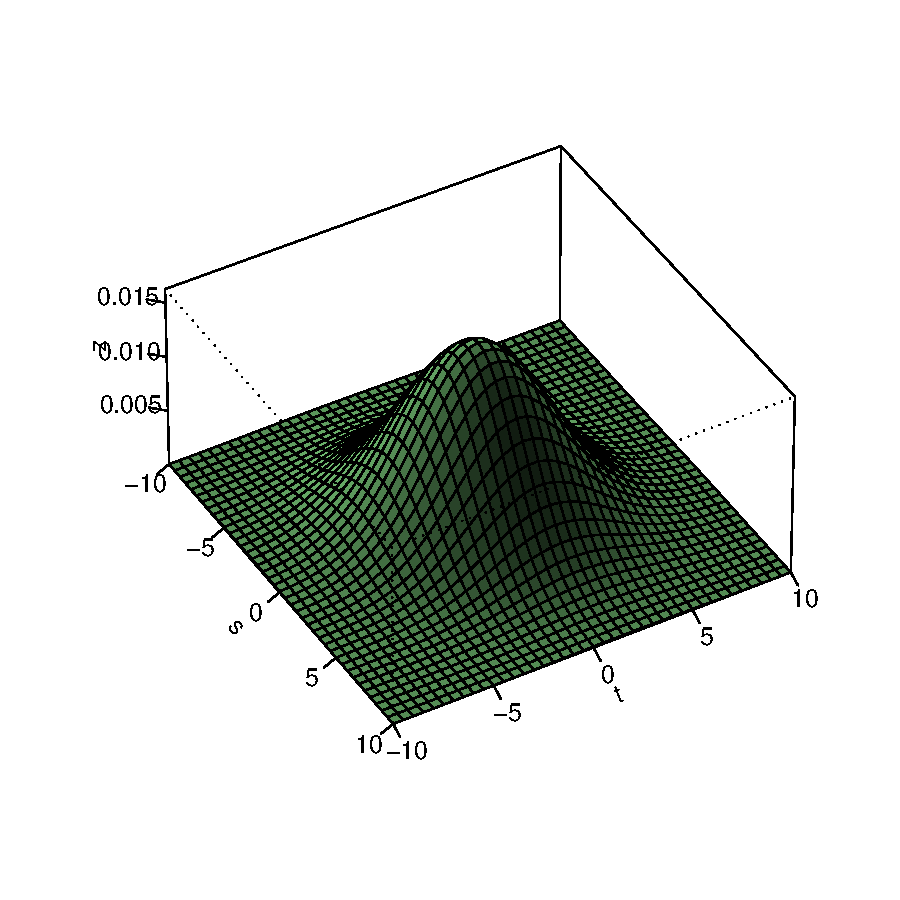
\includegraphics[width=4in]{Rho2.pdf}
}
\caption{Bivariate Normal Density, $\rho=0.2$}
\label{rho2}
\end{figure}

The surface is bell-shaped, though now in two dimensions instead of one.
Again, the height of the surface at any (s,t) point the relative
likelihood of $X_1$ being near s and $X_2$ being near t.  Say for
instance that $X_1$ is height and $X_2$ is weight.  If the surface is
high near, say, (70,150) (for height of 70 inches and weight of 150
pounds), it mean that there are a lot of people whose height and weight
are near those values.  If the surface is rather low there, then there
are rather few people whose height and weight are near those values.

Now compare that picture to Figure \ref{rho8}, with $\rho = 0.8$.

\begin{figure}
\centerline{
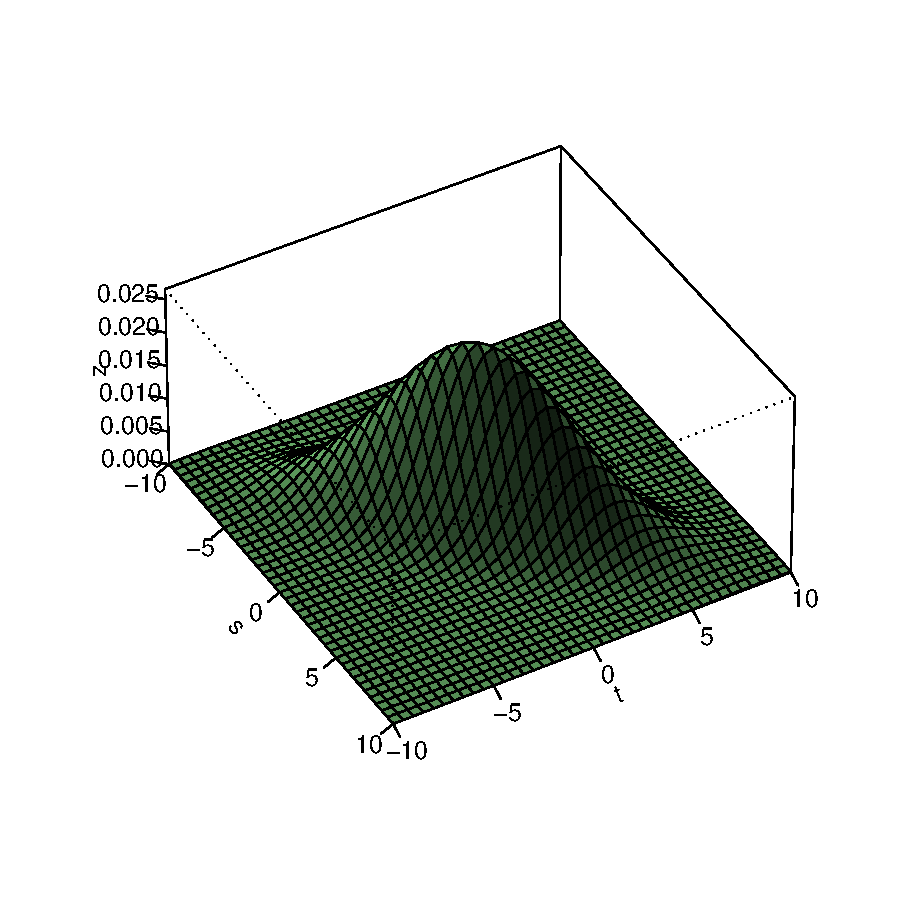
\includegraphics[width=4in]{Rho8.pdf}
}
\caption{Bivariate Normal Density, $\rho=0.8$}
\label{rho8}
\end{figure}

Again we see a bell shape, but in this case ``narrower.''  In fact, you
can see that when $X_1$ (s) is large, $X_2$ (t) tends to be large too,
and the same for ``large'' replaced by small.  By contrast, the surface
near (5,5) is much higher than near (5,-5), showing that the random
vector $(X_1, X_2)$ is near (5,5) much more often than (5,-5).

All of this reflects the high correlation (0.8) between the two variables.
If we were to continue to increase $\rho$ toward 1.0, we would see the
bell become narrower and narrower, with $X_1$ and $X_2$ coming closer
and closer to a linear relationship, one which can be shown to be

\begin{equation}
X_1 - \mu_1 = \frac{\sigma_1}{\sigma_2} (X_2 - \mu_2)
\end{equation}

In this case, that would be

\begin{equation}
X_1 = \sqrt{\frac{10}{15}} X_2 = 0.82 X_2
\end{equation}

\subsubsection{Properties of Multivariate Normal Distributions}
\label{mvnormproperties}

\begin{theorem}
\label{mvnormtheorem}

Suppose $X = (X_1,...,X_k)$ has a multivariate normal distribution with
mean vector $\mu$ and covariance matrix $\Sigma$.  Then:

\begin{itemize}

\item [(a)] The contours of $f_X$ are k-dimensional ellipsoids.  In the
case k = 2 for instance, where we can visualize the density of X as a
three-dimensional surface, the contours for points at which the bell has
the same height (think of a topographical map) are elliptical in shape.
The larger the correlation (in absolute value) between $X_1$ and $X_2$,
the more elongated the ellipse.  When the absolute correlation reaches
1, the ellipse degenerates into a straight line.

\item [(b)] Let A be a constant (i.e. nonrandom) matrix with k columns.
Then the random vector Y = AX also has a multivariate normal
distribution.\footnote{Note that this is a generalization of the
material on affine transformations on page \pageref{affine}.} 

The parameters of this new normal distribution must be $EY = A \mu$ 
and $Cov(Y) = A \Sigma A'$,  by (\ref{eaw}) and (\ref{covawaprime}).
   
\item [(c)] If $U_1,...,U_m$ are each univariate normal and they are
independent, then they jointly have a multivariate normal distribution.
(In general, though, having a normal distribution for each $U_i$ does
not imply that they are jointly multivariate normal.)  

\item [(d)] Suppose W has a multivariate normal distribution.  The
conditional distribution of some components of W, given other
components, is again multivariate normal.

\end{itemize}

\end{theorem}

Part [(b)] has some important implications:

\begin{itemize}

   \item [(i)] The lower-dimensional marginal distributions are also
   multivariate normal.  For example, if k = 3, the pair $(X_1,X_3)'$
   has a bivariate normal distribution, as can be seen by setting 

   \begin{equation} A = \left ( \begin{array}{ccc} 1 & 0 & 0\\ 0 & 0 & 1
   \end{array} \right )     \end{equation}

   in (b) above.
   
   \item [(ii)] Scalar linear combinations of X are normal.  In other
   words, for constant scalars $a_1,...,a_k$, set $a = (a_1,...,a_k)'$.
   Then the quantity $Y = a_1 X_1 +...+ a_k X_k$ has a univariate normal
   distribution with mean  $a' \mu$ and variance $a' \Sigma a$. 

   \item [(iii)] Vector linear combinations are multivariate normal.
   Again using the case k = 3 as our example, consider $(U,V)' =
   (X_1-X_3,X_2-X_3)$.  Then set

   \begin{equation}
   A = 
      \left (
      \begin{array}{ccc}
      1 & 0 & -1\\
      0 & 1 & -1   
      \end{array}
      \right )     
   \end{equation}

   \item [(iv)] The r-component random vector X has a multivariate normal
   distribution if and only if $c'X$ has a univariate normal
   distribution for all constant r-component vectors c.

\end{itemize}

In R the density, cdf and quantiles of the multivariate normal
distribution are given by the functions {\bf dmvnorm()}, {\bf pmvnorm()} 
and {\bf qmvnorm()} in the library {\bf mvtnorm}.  You can simulate a
multivariate normal distribution by using {\bf mvrnorm()} in the library
{\bf MASS}.

\subsubsection{The Multivariate Central Limit Theorem}

The multidimensional version of the Central Limit Theorem holds.  A sum
of independent identically distributed ({\it iid}) random vectors has an
approximate multivariate normal distribution.  Here is the theorem:

\begin{theorem}

Suppose $X_1, X_2, ...$ are independent random {\it vectors}, all having
the same distribution which has mean vector $\mu$ and covariance matrix
$\Sigma$.  Form the new random vector $T = X_1+...+X_n$.  Then for large
n, the distribution of T is approximately normal with mean $n \mu$ and
covariance matrix $n \Sigma$.

\end{theorem}


For example, since a person's body consists of many different
components, the CLT (a non-independent, non-identically version of it)
explains intuitively why heights and weights are approximately bivariate
normal.  Histograms of heights will look approximately bell-shaped, and
the same is true for weights.  The multivariate CLT says that
three-dimensional histograms---plotting frequency along the ``Z'' axis
against height and weight along the ``X'' and ``Y'' axes---will be
approximately three-dimensional bell-shaped.

The proof of the multivariate CLT is easy, from Property (iv) above.
Say we have a sum of iid random vectors:

\begin{equation}
S = X_1 + ... + X_n
\end{equation}

Then 

\begin{equation}
c'S = c'X_1 + ... + c'X_n
\end{equation}

Now on the right side we have a sum of iid {\it scalars}, not vectors,
so the univariate CLT applies!  We thus know the right-hand side is a
approximately normal for all c, which means $c'S$ is also approximately
normal for all c, which then by (iv) above means that S itself is
approximately multivariate normal.

\subsubsection{Example:  Finishing the Loose Ends from the Dice Game}

Recall the game example in Section \ref{dicegame}:

Suppose we roll a die 50 times.  Let X denote the number of rolls in
which we get one dot, and let Y be the number of times we get either two
or three dots.  For convenience, let's also define Z to be the number of
times we get four or more dots, though our focus will be on X and Y.
Suppose also that we win \$5 for each roll of a one, and \$2 for each
roll of a two or three.

Our analysis relied on the vector (X,Y,Z)' having an approximate
multivariate normal distribution.  Where does that come from?  Well,
first note that the exact distribution of (X,Y,Z)' is multinomial.  Then
recall (\ref{multinomsumindic}).  The latter makes (X,Y,Z)' a sum of
iid vectors, so that the multivariate CLT applies.

\subsubsection{Application:  Data Mining}
\label{datamining}

The multivariate normal family plays a central role in multivariate
statistical methods.  

For instance, a major issue in data mining is {\bf dimension reduction},
which means trying to reduce what may be hundreds or thousands of
variables down to a manageable level.  One of the tools for this, called
{\bf principle components analysis} (PCA), is based on multivariate
normal distributions.  Google uses this kind of thing quite heavily.
We'll discuss PCA in Section \ref{pca}.

To see a bit of how this works, note that in Figure \ref{rho8}, $X_1$
and $X_2$ had nearly a linear relationship with each other.  That means
that one of them is nearly redundant, which is good if we are trying to
reduce the number of variables we must work with.

In general, the method of principle components takes r original
variables, in the vector X and forms r new ones in a vector Y, each of
which is some linear combination of the original ones.  These new ones
are independent.  In other words, there is a square matrix A such that
the components of Y = AX are independent.  (The matrix A consists of the
eigenvectors of Cov(X); more on this in Section \ref{pca} of our unit on
statistical relations.

We then discard the $Y_i$ with small variance, as that means they are
nearly constant and thus do not carry much information.  That leaves us
with a smaller set of variables that still captures most of the
information of the original ones.

Many analyses in bioinformatics involve data that can be modeled well by
multivariate normal distributions.  For example, in automated cell
analysis, two important variables are forward light scatter (FSC) and
sideward light scatter (SSC).  The joint distribution of the two is
approximately bivariate normal.\footnote{See {\it Bioinformatics and
Computational Biology Solutions Using R and Bioconductor}, edited by
Robert Gentleman, Wolfgang Huber, Vincent J. Carey, Rafael A. Irizarry
and Sandrine Dudoit, Springer, 2005.}

